\documentclass[a4paper]{article}

%% Language and font encodings
\usepackage[english]{babel}
\usepackage[utf8x]{inputenc}
\usepackage[T1]{fontenc}

%% Sets page size and margins
\usepackage[a4paper,top=3cm,bottom=2cm,left=2cm,right=2cm,marginparwidth=1.75cm]{geometry}

%% Useful packages
\usepackage{amsmath}
\usepackage{graphicx}
\usepackage{algorithmic}
\usepackage{algorithm}
\usepackage[colorinlistoftodos]{todonotes}
\usepackage[colorlinks=true, allcolors=blue]{hyperref}

\title{A Data-Driven Approach to Imputation of Missing Gini Indices}
\author{Lingfeng Cheng, Mihir Paradkar, Yuting Tian}

\begin{document}
\maketitle



\section{Project Objective}
Worldwide, income inequality is a problem that leads to social unrest, economic stagnation, despair, and radical government changes. Accurate measures of this are indicative of a nation's health and its population's well-being, and provide governments and non-governmental organizations (NGOs) with the information they need to alleviate underlying issues. In particular, Gini indices are highly important since they are the gold standard for measuring wealth equity in an economic region. However, this metric requires income statistics that may be difficult to collect for war-torn countries or authoritarian regimes. The World Bank's World Development Indicators dataset contains the Gini coefficient and many other indicators of wealth equity for economic regions across more than 50 years. However, many Gini index measurements are missing which could provide vital information about historic income inequality in several places.

Given the importance of the Gini index and the high ratios of missing data, our project's objective is to fill in the missing Gini coefficients of the World Development Indicators (WDI) dataset by applying  Generalized Low Rank Models (GLRM). A Huber loss with a graph regularizer and a square regularizer is used as the objective function. Furthermore, a bootstrap framework is implemented to demonstrate the stability of the proposed imputation method. With more complete dataset provided by our project,corporations and governments could get better understanding and more accurate information of a country, which are important to make decisions and strategic plans.

\section{Dataset Description}
The WDI dataset is collected by the World Bank and updated quarterly. This dataset presents up-to-date and accurate global development data and covers a wide range of indicators like agriculture, the environment, education and infrastructure for every country and some aggregate regions in the world. Furthermore, for each perspective, a large number of indicators are proposed, with the corresponding data collected annually since 1960. These historical data augment the amount of information available to fit a model and also can help predict categories better by accounting for changes in indicators for particular regions. The numbers for each indicator are real-valued (no nominal or ordinal variables), but they are often on differing scales, with some indicators being strictly positive (number of doctors per capita, for example), some in very large scales (i.e. GDP being measured in billions of dollars), and some as percentages.

The ``WDI-data'' contains 52 columns and 372241 rows. The first four columns represent country name,country code,indicator name,indicator code and the rest of the columns are observations of all indicators ranging from 1960 to 2015. The first 66270 rows represent aggregate economic regions (i.e. Arab World), while the rest represent individual nations. While this dataset contains vast amounts of information on aspects of regional development and growth, it has some drawbacks relating to its dimensions and missing data. For example, many of the indicator values for years before 2000 are missing, and some indicators have no observed data at all.

Furthermore, certain columns are highly correlated, such as the GDP and GNP, which have a closed-form formulae relating one to the other. Additionally, the high dimensionality (1300-1500 columns) makes it difficult to visualize or reason about the effects of an individual indicator, reducing the interpretability of a fitted model. Also, in the raw dataset, each row represents a unique indicator-country pair whereas the columns represent years. This structure does not lend itself to analysis of the relationships between the indicators, so additional preprocessing was conducted.

The dataset distribution also contains auxiliary documentation files that document the shortened codes and abbreviations used to indicate the names of countries and indicators. Country codes are three-letter abbreviations for an economic region, while series codes are period-separated codes that categorize the indicators (i.e. AG.AGR.TRAC.NO is the number of agriculture machines), where the first two letters indicate topic, the second group is general subject, the third group is specific subject, and the last group is the specific extension.

Figure \ref{fig:m1}  is a histogram of the proportion of missing values in the dataset.
\begin{figure}
\centering
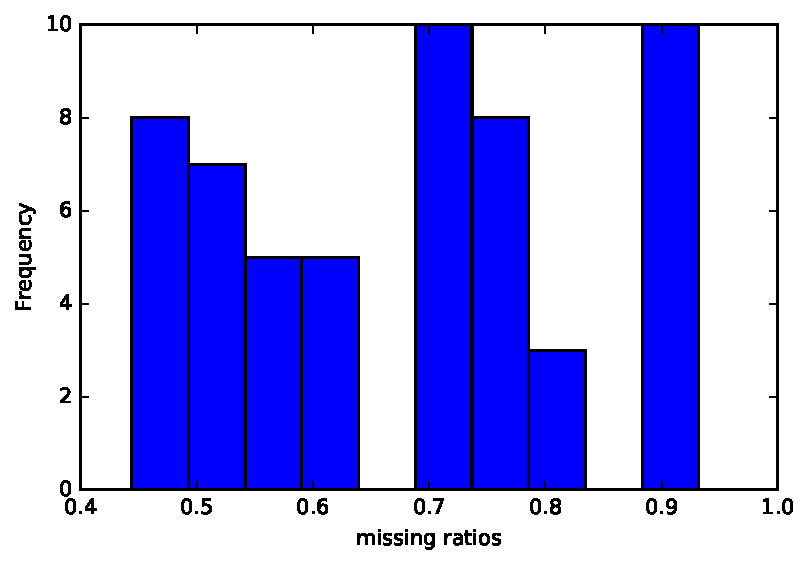
\includegraphics[width=0.6\textwidth]{missingRatio.pdf}
\caption{\label{fig:m1}The distribution of the ratio of missing values}
\end{figure}

The missing ratio ranges from 0.4 to over 0.9, making many statistical learning techniques difficult or impossible.

\section{Algorithm Development}
\subsection{Data Preprocessing}
To attempt to impute the Gini index, a subset over which the Gini index is measured is selected to perform the training and testing of our imputation methods. A specific standard is created for the data selection. Specifically, rows that contains the Gini index are selected and columns which are broadly related to the Gini index (columns starting with SI.* in the original dataset) are considered. The new subset contains 23 columns and 1265 rows, which represents the income and poverty indicators from 1960 to 2015. The training set is separated by choosing a random subset of 50\% of the observed values, and the test set is obtained as the rest of the values. The choice of this training to testing data ratio is to most accurately capture the real amount of missing data in the Gini index column.


\subsection{Generalized Low Rank Models}
The Generalized Low Rank Model (GLRM) is introduced to impute the missing values in the Gini index matrix. The model aims to minimize the difference between the observed values ($Y_{ij}$ and imputed values ($x_i^Tw_j$)) while imposing regularizations on both feature matrix $X$ and coefficient matrix $W$.
\begin{equation*}
\text{min}\quad \sum_{(i,j)\in \Omega}l_j(Y_{ij},x_i^Tw_j)+\sum_{i=1}^nr_i(x_i)+\sum_{j=1}^dr_j(w_j)
\end{equation*}
In this project, the following Huber loss is chosen as the loss function due to its robustness in handling outlier values. 
\begin{equation*}
\text{Huber}(z)=\begin{cases}
\frac{1}{2}z^2,&\text{if $|z|\leq1$}\\
|z|-\frac{1}{2},&\text{if $|z|>1$}
\end{cases}
\end{equation*}
where $z=Y_{ij}-x_i^Tw_j$.\\
A square regularizer is selected for the coefficient matrix $w$ which indicates a preference over small coefficients. An exotic graph based regularizer is used for the feature matrix $X$, and is further illustrated in Section 3.3.
\subsection{A graph regularizer for the feature matrix}
The motivation of using a graph regularizer on the feature matrix is based on the matrix's inherent temporal correlation. Specifically speaking, since the Gini index is collected annually from 1960 to 2015, the temporal correlation between the neighboring years justifies the need for an adjacency matrix. The addition of the adjacency matrix relaxes the assumption that the observations are i.i.d. and instead brings together the values for consecutive years in a given region. This way, our model accounts for temporal fluctuations across countries but penalizes large changes in features of consecutive years.

Instead of the adjacency matrix, however, the regularizer used in this experiment uses the Laplacian matrix, defined as the degree matrix minus the adjacency matrix. Since the subset of the dataset we use has several examples missing, the graph matrix is constructed by connecting any pair of observations with consecutive years and the same region with an edge. Then the Laplacian matrix is calculated from the resulting graph structure. Pseudocode for this graph construction is below, assuming that data is sorted by country and year:

\begin{algorithm}
\caption{Graph Construction}
\begin{algorithmic}[1]
\FOR{i in 1 to (rows(wdi) - 1)}
\IF{$wdi_i.country$ == $wdi_{i+1}.country$}
\IF{$wdi_{i+1}.year$ == $wdi_i.year + 1$}
\STATE add (i,i+1) as an edge to the graph
\ENDIF
\ENDIF
\ENDFOR
\end{algorithmic}
\end{algorithm}


Using this graph, a low rank model is fitted using the alternating-update proximal gradient method.

\subsection{Proximal gradient method}
Once the loss functions and the regularizers have been determined, the proximal gradient method can be used to simultaneously solve the coefficient matrix $W$ and feature matrix $X$ using alternating updates. In this case, the matrix $W$ represents the loading on each column and the matrix $X$ is the weights of each loading on a given observation, so the graph smoothing is applied to the different examples of $X$. That is, each row of $X$ corresponds to a country/year pair and its entries are linear combinations of the original features. Furthermore, each column of $W$ is the mapping from this compressed space back to a column of the original dataset. Once the value of the regularization penalty and the proximal operator of the regularization function are known, then alternating proximal gradient updates will converge. In the case of the graph regularizer, the value of the graph regularizer is given by 
\begin{equation*}
rx(X) = tr(X^T L X)
\end{equation*}
where $L$ is the graph Laplacian matrix. To derive the update algorithm for $X$, let $\alpha$ be the stepsize and let
\begin{equation*}
U = X - \alpha\nabla_X(\sum_{(i,j)\in \Omega}l_j(Y_{ij},x_i^Tw_j))
\end{equation*}
The proximal operator is defined as:
\begin{equation*}
\text{prox}_r(U) = \text{argmin}_{X_{t+1}}( \alpha r(X_{t+1}) + \frac{1}{2}\|U - X_{t+1}\|_F^2)
\end{equation*}
This can then be found for $\text{prox}_{rx}$. Using the fact that $\nabla_X rx(X) = 2LX$, setting the gradient of the proximal expression to zero and solving for $U$ gives that:
\begin{equation*}
X_{t+1} = \text{prox}_{rx}(U) = (2\alpha L + I)^{-1}U
\end{equation*}
where $I$ is the identity matrix of the same size as $L$. 

However, using the Laplacian regularizer on X is not sufficient to ensure convergence, as $L$ is not necessarily invertible. 
% The reason behind this is that for some invertible transformation $Q$ that scales the components of $X$ in the kernel of $L$ by some $\alpha > 1$ while preserving the component of $X$ in the image of $L$, $tr(X^TQ^TLQX)$ is the same as $tr(X^TLX)$ while $\|YQ^{-1}\|_F^2$ decreases. This causes the Frobenius norm of $Y$ to decrease to zero while the Frobenius norm of $X$ increases without bound.

To remedy this issue, we defined
\begin{equation*}
M = L + \beta I
\end{equation*}

where $\beta$ introduces a small amount of quadratic regularization. This is the case because
\begin{equation*}
tr(X^TMX) = tr(X^TLX) + \beta\|X\|_F^2
\end{equation*}

Using the property that a positive semi-definite matrix added to a multiple of the identity is positive definite and invertible, this now provides sufficient constraint to converge properly.

After making the adjustment to the Laplacian matrix, the new update algorithm is given by:
\begin{equation*}
X_{t+1} = \text{prox}_{rx}(U) = (2\alpha(L + \beta I) + I)^{-1}(U)
\end{equation*}

Since the update algorithm for quadratically-regularized $W$ is:
\begin{equation*}
W_{t+1} = \frac{V}{1 + 2\alpha}
\end{equation*}
where
\begin{equation*}
V = W_t - \nabla_W (\sum_{(i,j)\in \Omega}l_j(Y_{ij},x_i^Tw_j))
\end{equation*}
there exists an alternating update sequence that converges.
However, in practice, the standard Low Rank Models package by Udell et al. assumes that regularization is applied to individual rows, not to the whole matrix. This meant that we required a re-implementation of GLRMs that allowed for whole-matrix updates, which include the proximal gradient updates that we require for the graph regularizer.

\subsection{Validation and Experiment Design}
In each trial, the observation set is restricted to half of the observed entries, causing about 60\% of the Gini indices to be in the observation set and 40\% to be left for imputation. Throughout the whole project, the square relative deviance (Defined below) is calculated as the error metric. 
\begin{equation*}
\text{SRE} = \frac{(\text{imputed}-\text{actual})^2}{\text{actual}^2}
\end{equation*}
And the error for both the training set and test set is calculated as:
\begin{equation*}
\text{error}_i=\frac{1}{S_i}\sum_{i}\text{SRE}_{j\in i}
\end{equation*}
where $i=\{\text{training},\text{test}\}$, $j$ is the data point in the set $i$, and $S_i$ is the size of the set $i$.

To find the most appropriate rank for the model, a baseline low-rank model is firstly fitted. This baseline model is defined as 
\begin{equation*}
\text{min}\quad \sum_{(i,j)\in \Omega}\text{Huber}_j(Y_{ij},x_i^Tw_j)+\sum_{i=1}^n||x_i||^2+\sum_{j=1}^d||w_j||^2
\end{equation*}
A series rank values, i.e. 2, 5, 10, and 20, are experimented, from which the value provides least test error is chosen.

In the next step, the magnitude of the graph regularization model, $\alpha$, is determined by fitting the low rank model defined in Section 3.2 while fixing the optimal rank value selected from the previous baseline model.

Finally, to ensure this algorithm is insensitive to different samples, different training and testing sets are resampled from the same dataset. For each new sample, a baseline and a graph-regularized model are fitted with the previously determined optimal combination of hyper-parameters. The accuracy of the baseline and the graph-regularized models are compared over the two new replications. 


\section{Result Analysis}
\subsection{Hyper-parameter Determination}
To determine the optimal rank value for the Generalized Low Rank Model, the testing error has been calibrated for a series of rank values, i.e. 2, 5, 10, and 20. Figure \ref{fig:rank} represents a typical trend of bias-variance trade-off. As the rank value increases from 2 to 10, both the training and testing error decreases due to the increase of model complexity. However, as the rank value increases from 10 to 20, these two errors increases as a result of increased model variance. Therefore, rank 10 is chosen as the optimal hyper-parameter.
\begin{figure}
\centering
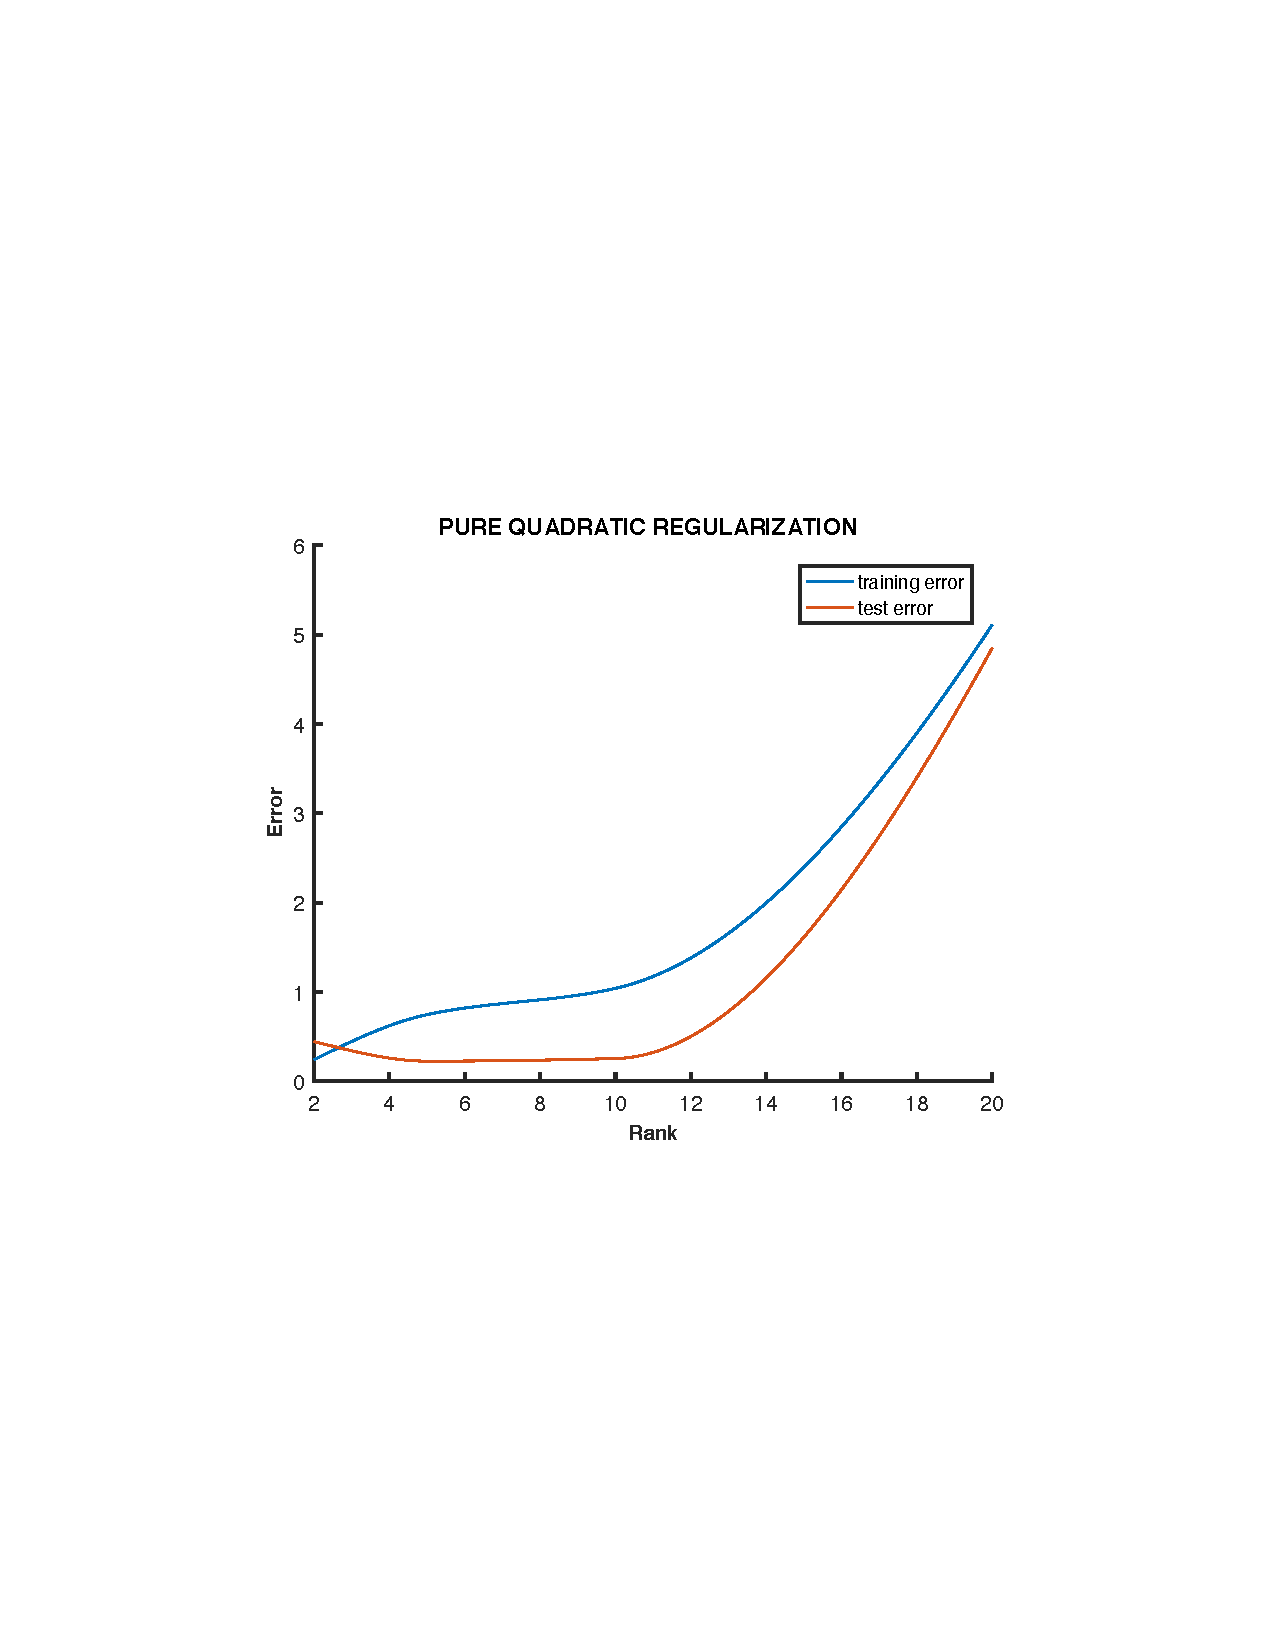
\includegraphics[width=0.6\textwidth]{PURE_QUADRATIC_REGULARIZATION.pdf}
\caption{\label{fig:rank}The training and testing errors for different rank values}
\end{figure}

To determine the optimal magnitude $\alpha$ of the graph regularizer, a series of values ranging from 0 to 5 have been tested. Although the magnitude of 2 achieves the minimum training error, 3 is chosen to be the magnitude due to considerably lower testing error.
\begin{figure}
\centering
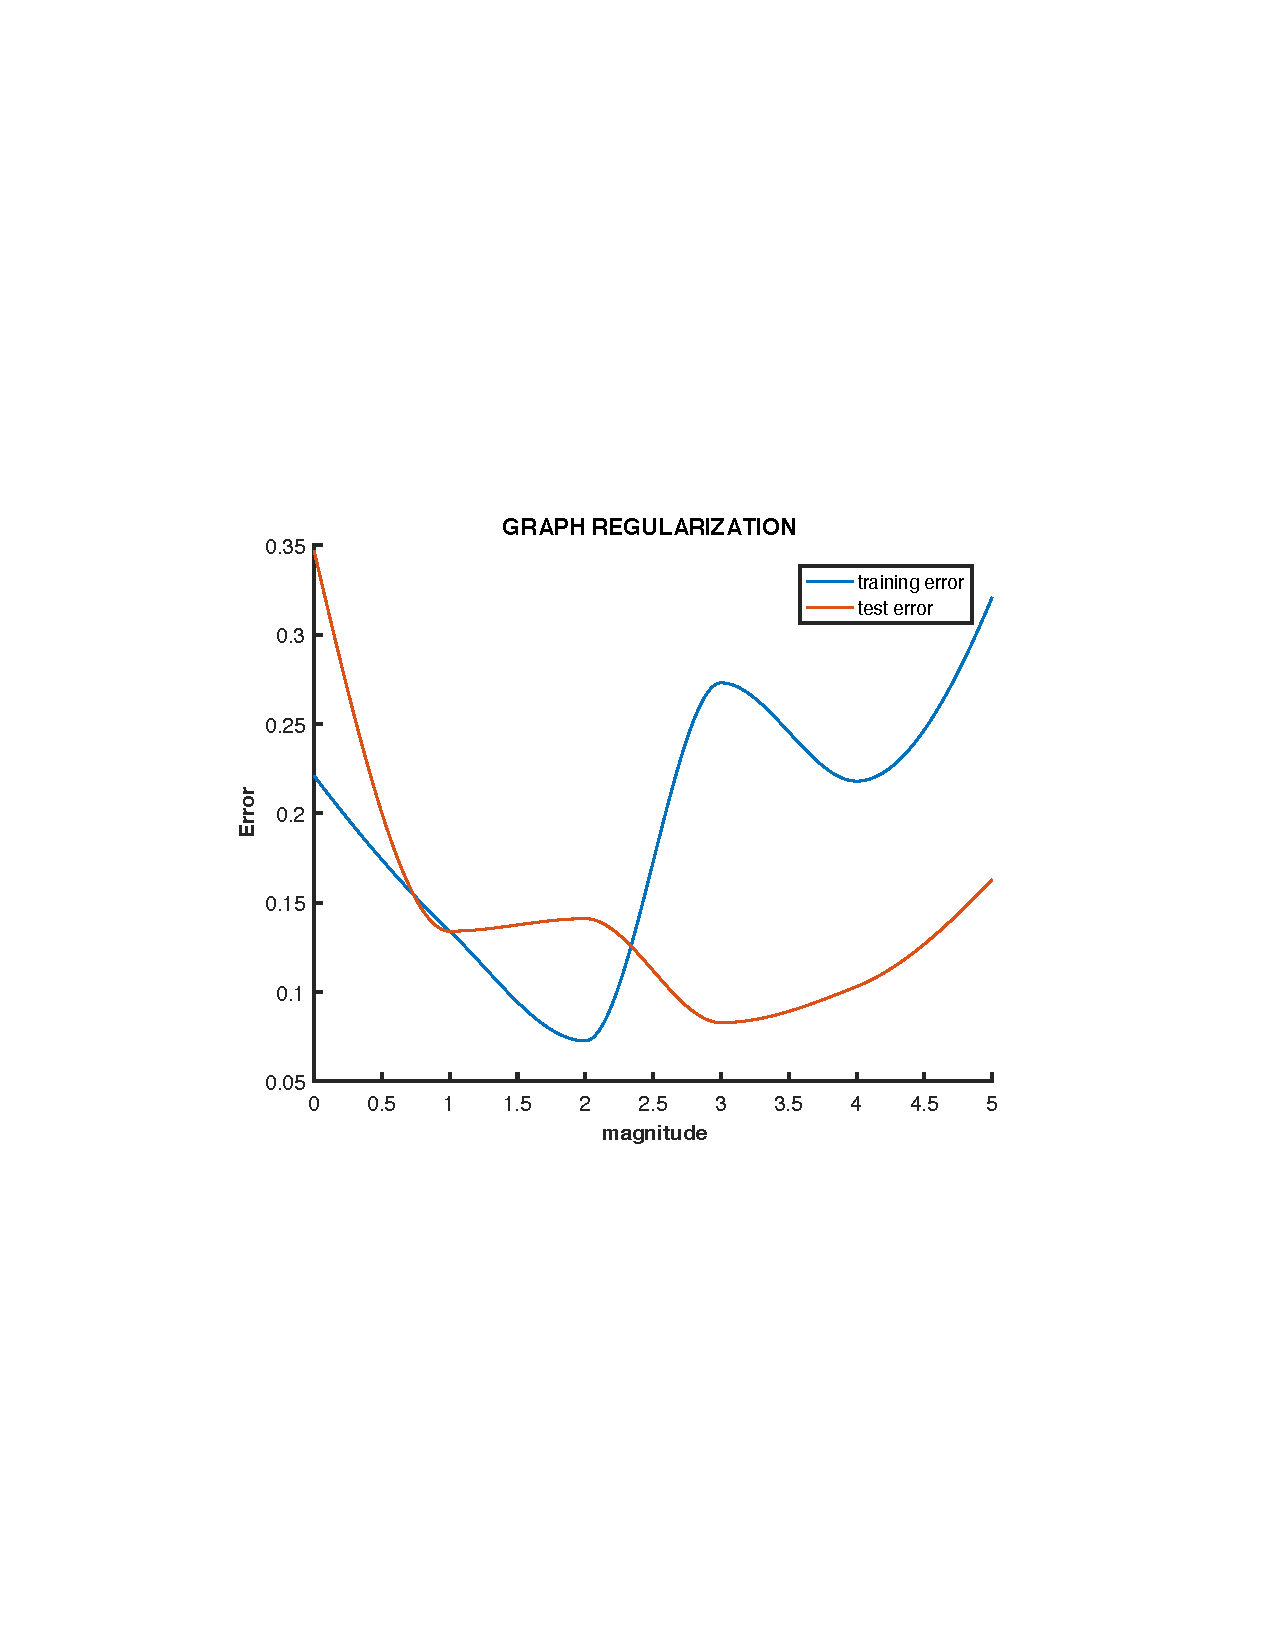
\includegraphics[width=0.6\textwidth]{GRAPH_REGULARIZATION.pdf}
\caption{\label{fig:graph}The training and testing errors for different magnitudes of the graph regularizer}
\end{figure}
\subsection{Test Error Distribution}
Furthermore, the distribution of the square relative errors for all the entries in the test set has been plotted in Figure \ref{fig:hist}. The vast majority errors are less than 0.05, which further substantiates the choice of hyper-parameters and the implementation of the algorithm. 
\begin{figure}
\centering
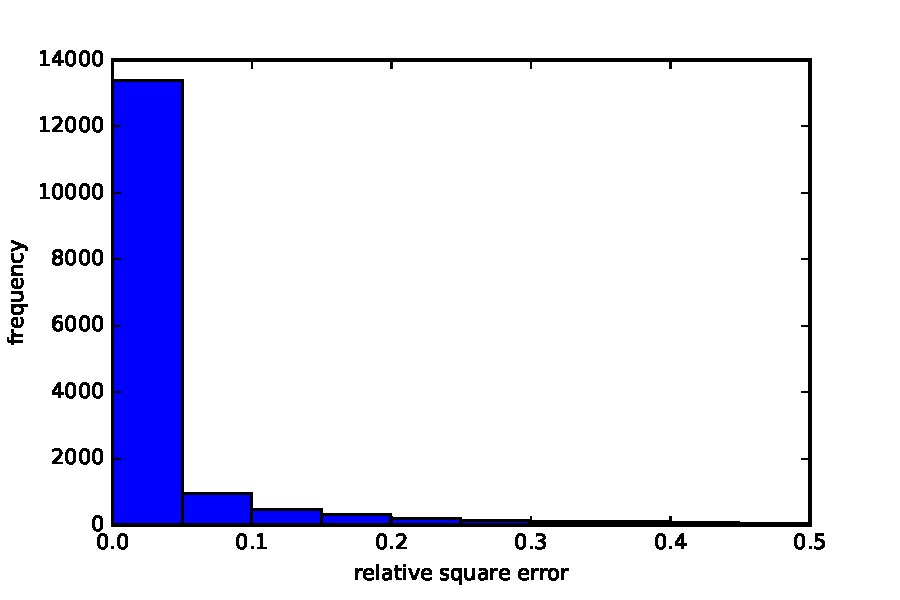
\includegraphics[width=0.6\textwidth]{hist.pdf}
\caption{\label{fig:hist}The square relative error distribution for the test set}
\end{figure}
\subsection{Replicate Analysis }
To further validate the correctness of the model, two additional samples have been created from the original dataset. Due to the large amount of missing data, even within the subset that is evaluated, changing sampling indices could mean that there are no observations for entire columns, which drastically increase variance over the dataset. 

Both the training and the validation errors for the regularized model have been compared with the baseline model, where a quadratic regularizer is used on matrix $X$ instead of the graph Laplacian regularizer. The results are listed in Table \ref{tab:compare}. Throughout the two samples, both the training and the validation error decrease after the graph regularizer is introduced. Therefore, it is valid to conclude the graph regularizer consistently performs as well as or better than our baseline, even though the sampling methods cause the error to vary widely depending on the chosen training indices.

\begin{table}
\centering
\begin{tabular}{|c|c|c|c|c|}
\hline
 & sample 1 & baseline 1 & sample 2 & baseline 2\\\hline
Training Error & 0.336 & 0.552 & 0.0697 & 0.118\\
Validation Error & 0.638 & 0.552 & 0.118 &4.14
\end{tabular}
\caption{Accuracy comparisons of different samples}
\label{tab:compare}
\end{table}
\section{Conclusion and Further Experiments}
The results of this project demonstrate that Generalized Low-Rank Models can impute values on highly sparse datasets with very little error. Specifically, the addition of graph-Laplacian regularization and a robust loss function can significantly reduce the error on unobserved entries of a dataset, even when supervised learning algorithms fail. Further experimentation could use a graph connecting similar countries as well as similar indicators to utilize more information from other metrics, countries, and times in imputing missing data. Given the difficulty of measuring indices like the Gini coefficient, reliable estimates for historical values can prove very useful to government and organizations looking to combat poverty and economic crisis. Although imputation is no substitute for determined data collectors, our method can prove crucial when it is unsafe or impossible for any organization to obtain vital information.
\end{document}